\begin{figure}[!h]
    \centering
    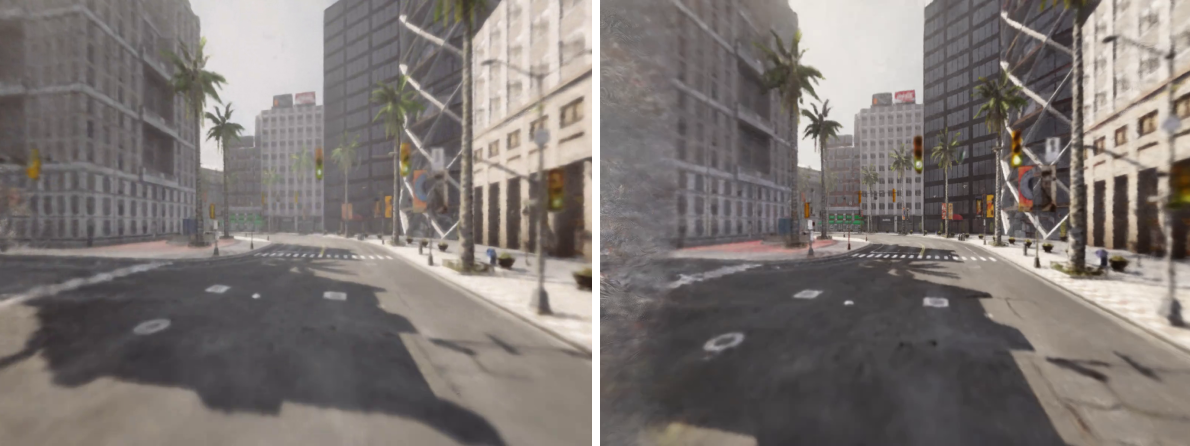
\includegraphics[width=1.0\textwidth]{figures/block-nerf-frame-comparison.png}
    \caption{Comparison of two consecutive frames of a single render on a 12 block NeRF. The first frame (left) is the last frame rendered by block number 1. The second frame (right) is the first frame rendered by block number 2. The details of the scenery in the second frame is clearly better than the first, which is expected as block number 2 have been trained on close-up images of the scene. This difference could be mitigated by looking into image merging techniques such as inverse distance weighing.}
    \label{fig:block-nerf-frame-comparison}
\end{figure}